\setlength{\droptitle}{-4\baselineskip} % Move the title up
\pretitle{\begin{center}\Huge\bfseries} % Article title formatting
    \posttitle{\end{center}} % Article title closing formatting
\title{Milites} % Article title
\author{
  \textsc{Luigi Russo, Matteo Salvino}\\[1ex] % Authors
  \normalsize Sapienza University of Rome \\ % Your institution
}
\date{\today} % Leave empty to omit a date

\renewcommand{\maketitlehookd}{
  \begin{minipage}{\linewidth}
    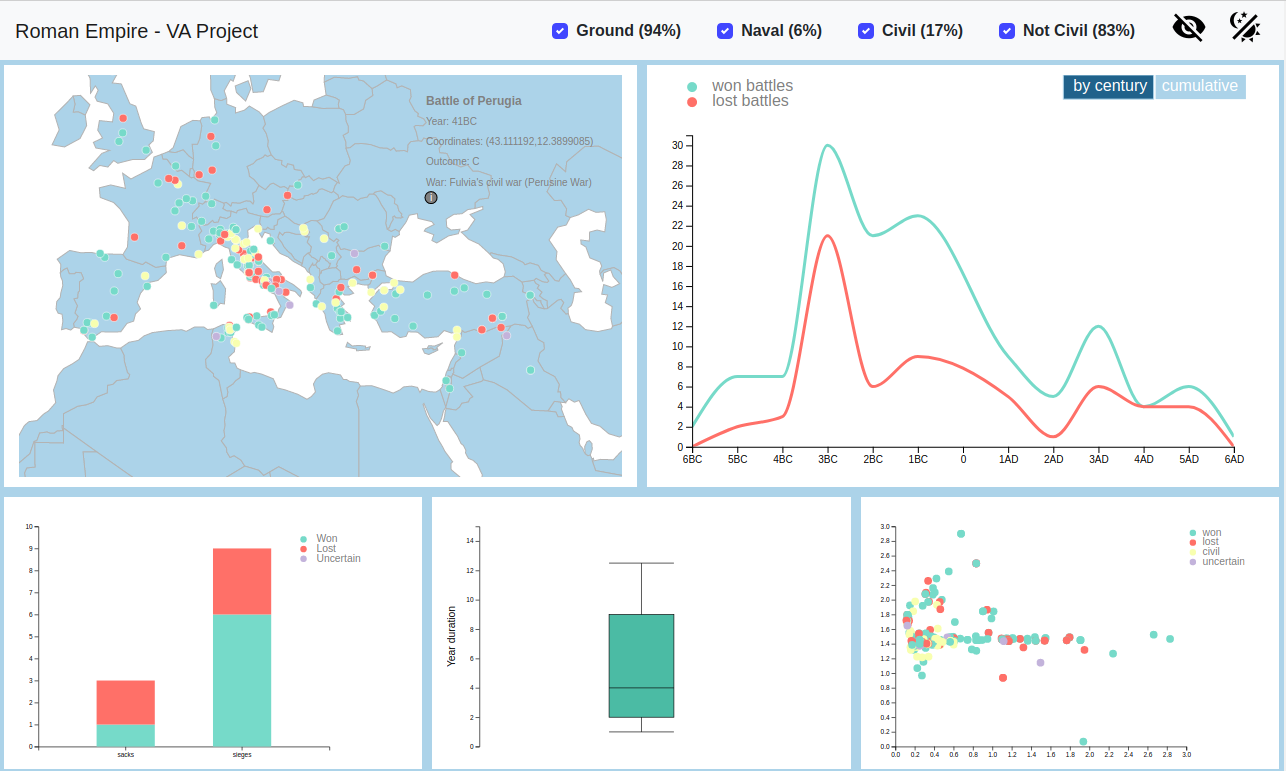
\includegraphics[width=\linewidth]{./images/visualization_views.png}
    \captionof{figure}{Visualization with light mode enabled and blind safe mode disabled}
  \end{minipage}

  \begin{abstract}
    \noindent The military of ancient Rome is unanimously considered a key element in the rise of Rome. We developed a visual analytics tool for educational purposes, mainly to give a visual representation of ancient Roman battles and wars. The multiple interactive views of our project present high level features, but the user also has the possibility to explore further information, e.g. via references link associated to each battle.
  \end{abstract}
}
